\section{Preliminary Study: Understanding How Stencil Patterns Affect Prediction-based Lossy Compression Performance}\label{sec:preliminary study}

% 在这一章中。。。
% 需要补充：从这里开始所有的实验和理论（除了第四章最后一个subsection）都是在单轮预测中的。因为每一轮预测实际上并不能区分它的参考点是已压缩的还是未压缩的，对于预测器来说只是特征/相关性不同的数据而已。

\subsection{Key Concepts in SZ Compression Framework}
% 你在这里介绍一下prediction，尤其是interpolation。因为你的stencil pattern和reference points其实都是基于interpolation来做的。如果reviewer不懂interpolation，他直接看后面的概念会比较头大。所以先介绍一下比较好。

% 在这一章中我们详细介绍一下SZ compression framework，并定义一些重要的概念。
% 在xxx章中，我们提到过，SZ 框架包含预测、量化、压缩三步。预测器可以认为是一个加权和操作，我们作出以下定义：
% 预测目标：预测器想要预测出的那个数
% 参考点：预测器能够访问的数的集合
% stencil pattern: 所有参考点相对于预测目标的位置
% coefficients: 计算加权和时，每个参考点的权重

% stencil pattern 和 coefficients可以描述一个基于加权和的预测器，SZ1、SZ3、QoZ使用的预测器都属于这一类中的比较特殊的一种，即它们的系数是根据插值公式计算出来的。这一章接下来的部分中，我们展示的是穷举coefficients后得到的最优结果。

Recall that we briefly reviewed the SZ compression framework~\cite{liang2022sz3} in Figure~\ref{fig:sz3 diagram}. 
Here, we introduce several key concepts used throughout this section.
The SZ framework consists of three stages: prediction, quantization, and lossless encoding. 
In this work, we specifically focus on interpolation-based predictors~\cite{zhao2021optimizing}, which achieve strong compression performance in practice~\cite{liu2022dynamic,liu2024high}. 
Such predictors estimate each data point as a weighted combination of neighboring values.
Specifically, we define the following concepts:

\begin{itemize}
\item \textbf{\textit{Prediction Target}}: The data point to be predicted.
\item \textbf{\textit{Reference Points}}: The set of data points accessible to the predictor for predicting values of the prediction target.
\item \textbf{\textit{Stencil Pattern}}: the relative positions of all reference points with respect to the prediction target.
\item \textbf{\textit{Coefficients}}: The weights assigned to each reference point in the weighted sum.
\end{itemize}

If the prediction target is $T$, reference points are $\{R_1, ..., R_n\}$, and their corresponding coefficients are $\{c_1, ..., c_n\}$. The coefficients should satisfy $\sum_{i=0}^nc_i=1$.

Together, the stencil pattern and coefficients fully characterize a weighted-sum predictor. The predictors used in SZ3~\cite{zhao2021optimizing,liang2022sz3}, and QoZ~\cite{liu2022dynamic,liu2024high} can be viewed as specific instances of this formulation, where the coefficients are derived from interpolation schemes. In principle, other choices of coefficients can also be used during prediction.
In the following part of this section, we investigate the impact of stencil patterns on compression performance and present the best results obtained by iterating over the coefficient space.


\subsection{General Stencil Patterns}
% 介绍一下stencil pattern是什么，有哪些比较常见的stencil patterns（并且参与了你的测试，不管有没有用，只要你测试过的都介绍一下）。同时，你要介绍一下什么是reference point。
% 这里可以加几个interpolation的图。

% SZ3的stencil pattern是比较常用的。SZ3有linear和cubic两种1维预测器，分别对应包含2个和4个点的stencil pattern。不过linear 预测器可以理解为修改过参数的cubic预测器。
% 两种常见的、包含4个stencil pattern的、2D的predictor
% QoZ使用过
% 理论上来说，可以有更高维的predictor、访问更多参考点，比如说。。。

The stencil patterns used in SZ3 are representative and widely adopted in practice. SZ3 provides two one-dimensional predictors, namely linear and cubic interpolation, which can be shown in Figure~\ref{fig:general sp} (a) and (b). They correspond to stencil patterns involving two and four reference points, respectively. Notably, the linear predictor can be viewed as a special case of the cubic predictor, since its reference points form a subset of those used in the cubic predictor.

\begin{figure}[htb]
    \centering
    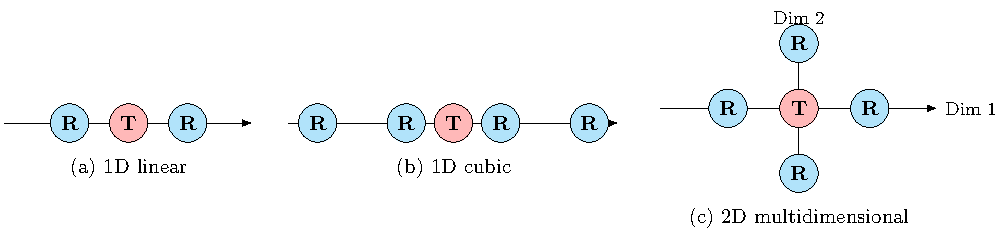
\includegraphics[width=0.9\linewidth]{revised-fig/1-sz-qoz-predictors.pdf}
    \caption{Interpolation predictors used in SZ3 and QoZ.}
    \label{fig:general sp}
\end{figure}

Some two-dimensional stencil patterns involving four reference points are also commonly used, as explored in QoZ~\cite{liu2022dynamic}. 
Two examples can be found in Figure~\ref{fig:general sp} (c) and (d).
In principle, more general predictors can be constructed by extending these designs to higher dimensions or by incorporating more reference points. Such extensions further enlarge the predictor design space and provide additional flexibility to capture complex data correlations within a scientific data domain.


\subsection{Stencil Patterns on Compression Performance}
\label{sec:stencil-patterns-performance}
% 总而言之，这一块是为了证明,同样reference point的情况，2D或者higer-dimensional stencil pattern没啥用，1D的就够了。
% 简而言之，得到takeaway1: 1D stentil pattern就够用了！

% 更多reference point可能会导致一些代价，包括每次运行的速度更慢，以及predictor中需要tune的coefficients更多。所以公平比较stencil pattern的话，需要限定在相同数量的reference point。
% 如果存在可以利用的高维信息，一维四点预测可以利用，而二维四点预测用不了
% 如果不存在可以利用的高维信息，可变参数的一维四点预测可以退化为一维两点预测，不会受到杂乱高维信息的干扰，因此不会弱于二维四点预测。
% 模拟最后一轮预测，用真实值预测真实值（在实际的预测中用的是压缩后的值，但终究是每个点上一个数，问一下ai这里怎么写）
In this section, we compare one-dimensional and two-dimensional predictors to understand their relative effectiveness in compression.
For a fair comparison, we fix the number of reference points used by each predictor.
While increasing the number of reference points may affect compression performance, it inevitably introduces higher computational and tuning overhead.
For the stencil patterns shown in Figure~\ref{fig:general sp}(b) and (c), we introduce a tunable variable $v$ to ensure that the coefficients sum to 1.
The computation for (b) is illustrated in Figure~\ref{fig:general sp coeff}, and (c) follows the same formulation, but just in a different direction.

% 对于figure2的（b）和（c）这两种stencil pattern，我们设计如图X的可变参数，它们都有一个未知量。对于可变参数的一维四点加权预测器，参数t负责控制。。。，在【3/16,6/16】之间遍历。当t=4/16时，这个预测器变成了一维一阶插值，当t=5/16时，这个预测器变成了一维三阶插值。对于可变参数的二维一阶插值，参数t负责控制预测器更多的利用哪个维度上的信息，在【-3/32,3/32】之间遍历。当t=0时，两个维度上的信息有相同的权重。Figure2的（a）是一维四点预测器的一种特殊情况。Figure2的（d）将会在之后单独讨论。



\begin{figure}
    \centering
    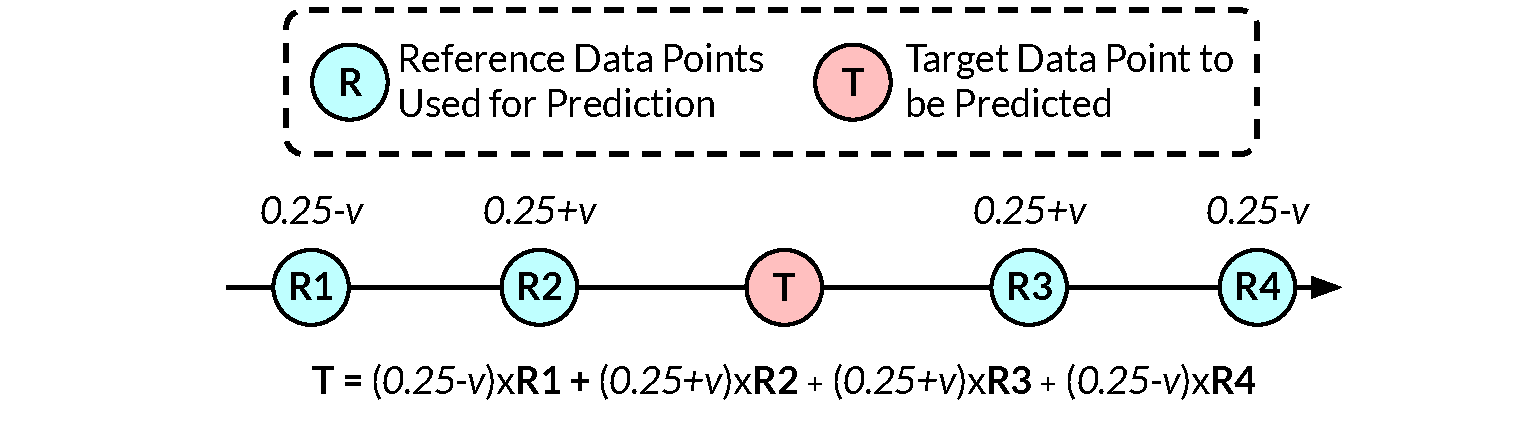
\includegraphics[width=1\linewidth]{revised-fig/2-coefficients-and-tunable-variables.pdf}
    \caption{Illustrating coefficients of a 1D four-point predictor and how they are calculated to predict the target. The 2D four-point predictors work similarly but in a different stencil pattern (e.g., Figure~\ref{fig:general sp}) (c) and (d). $v$ here denotes a tunable variable.}
    \label{fig:general sp coeff}
\end{figure}

% For the 1D four-point predictor (Figure~\ref{fig:general sp coeff}), $v\in\left[\frac{3}{16},\frac{6}{16}\right]$ controls the relative contribution of neighboring samples. Existing linear and cubic interpolation predictors correspond to the special cases when $v=\frac{4}{16}$ or $\frac{5}{16}$.
% For the 2D four-point predictor (the stencil pattern is Figure~\ref{fig:general sp} (c)), $b\in\left[-\frac{3}{32},\frac{3}{32}\right]$ controls the relative emphasis between the two spatial dimensions. When $t=0$, the two dimensions are assigned equal importance.

For the 1D four-point predictor (Figure~\ref{fig:general sp coeff}), the parameter $v \in \left[\frac{3}{16}, \frac{6}{16}\right]$ controls the contribution of neighboring samples.
Existing linear and cubic interpolation predictors correspond to the special cases $v=\frac{4}{16}$ and $v=\frac{5}{16}$, respectively.
For the 2D four-point predictor (Figure~\ref{fig:general sp}(c)), the parameter $v \in \left[-\frac{3}{32}, \frac{3}{32}\right]$ controls the balance between the two spatial dimensions.
When $v=0$, both dimensions are treated equally.

% Figure 2(a) corresponds to a special case of the 1D four-point predictor. Figure 2(d) will be discussed separately in a later section.

% 以三维数据为例，此时一维四点和二维四点预测器都有3个可能的方向。按照以往压缩器总结的经验，三阶插值预测器在少数情况下，比如高阶信息由大量噪声时，会比一阶插值更差。然而，可变参数的一维四点预测器（Figure3（a））可以放弃使用较远的两个reference point，从而避免高阶信息中的噪声的负面影响。所以最好的一维四点预测器通常不会弱于最好的三维四点预测器。
% 另一方面来说，当存在可以利用的高阶信息时，二维四点预测器不能利用这些信息，（接下来大概要说沿着每个维度进行线性插值的误差被叠加，不同维度上的残差大致无关。从数学期望上来讲，如果分配恰当的权重，叠加后的误差应该比叠加前更集中。但也正因为叠加的是相互无关的residuals，预计效果不如一维四点预测。）

% Taking 3D data as an example, both predictors in Figure~\ref{fig:general sp coeff} can be applied along three possible directions. Empirically, traditional cubic interpolation may perform worse than linear interpolation in certain cases, especially when high-order information is dominated by noise. In contrast, the tunable 1D four-point predictor can discard the two farther reference points, thereby mitigating the adverse impact of noisy high-order components. As a result, the best 1D four-point predictor is typically no worse than the best 2D four-point predictor.

% On the other hand, when useful high-order information is present, the 2D four-point predictor is unable to exploit it. Instead, it performs interpolation independently along each dimension, and the resulting residuals from different dimensions are approximately uncorrelated. From an expectation perspective, combining these residuals with appropriate weights may lead to a more concentrated error distribution. However, since the combined residuals originate from largely independent sources, the achievable gain is limited, and the overall performance is expected to be inferior to that of the 1D four-point predictor.

We analyze the relative behavior of 1D and 2D four-point predictors under different data characteristics.
\begin{itemize}
\item \textit{Case 1: Noisy or weak high-order structures}

When high-order information is dominated by noise, predictors that rely on distant reference points may introduce large prediction errors.
For example, cubic interpolation uses higher-order neighbors and can be sensitive to noise.
In contrast, the tunable 1D four-point predictor can reduce the contribution of distant points, effectively adapting to simpler local patterns.

\item \textit{Case 2: Data with useful high-order information}

When meaningful high-order structures are present, 1D predictors can more effectively capture high-order correlations. In contrast, 2D predictors perform interpolation independently along each dimension.
The resulting residuals from different dimensions are therefore weakly correlated.
Combining such residuals may reduce variance to some extent, but the gain is limited due to the lack of cross-dimensional coupling.
As a result, these predictors may not fully exploit structured correlations in the data.

\end{itemize}





% 要不要在这里说1D四点预测其实是在尝试将两种不同方式统计出的二次项相互抵消？（要写）

\begin{figure}[htb]
    \centering
    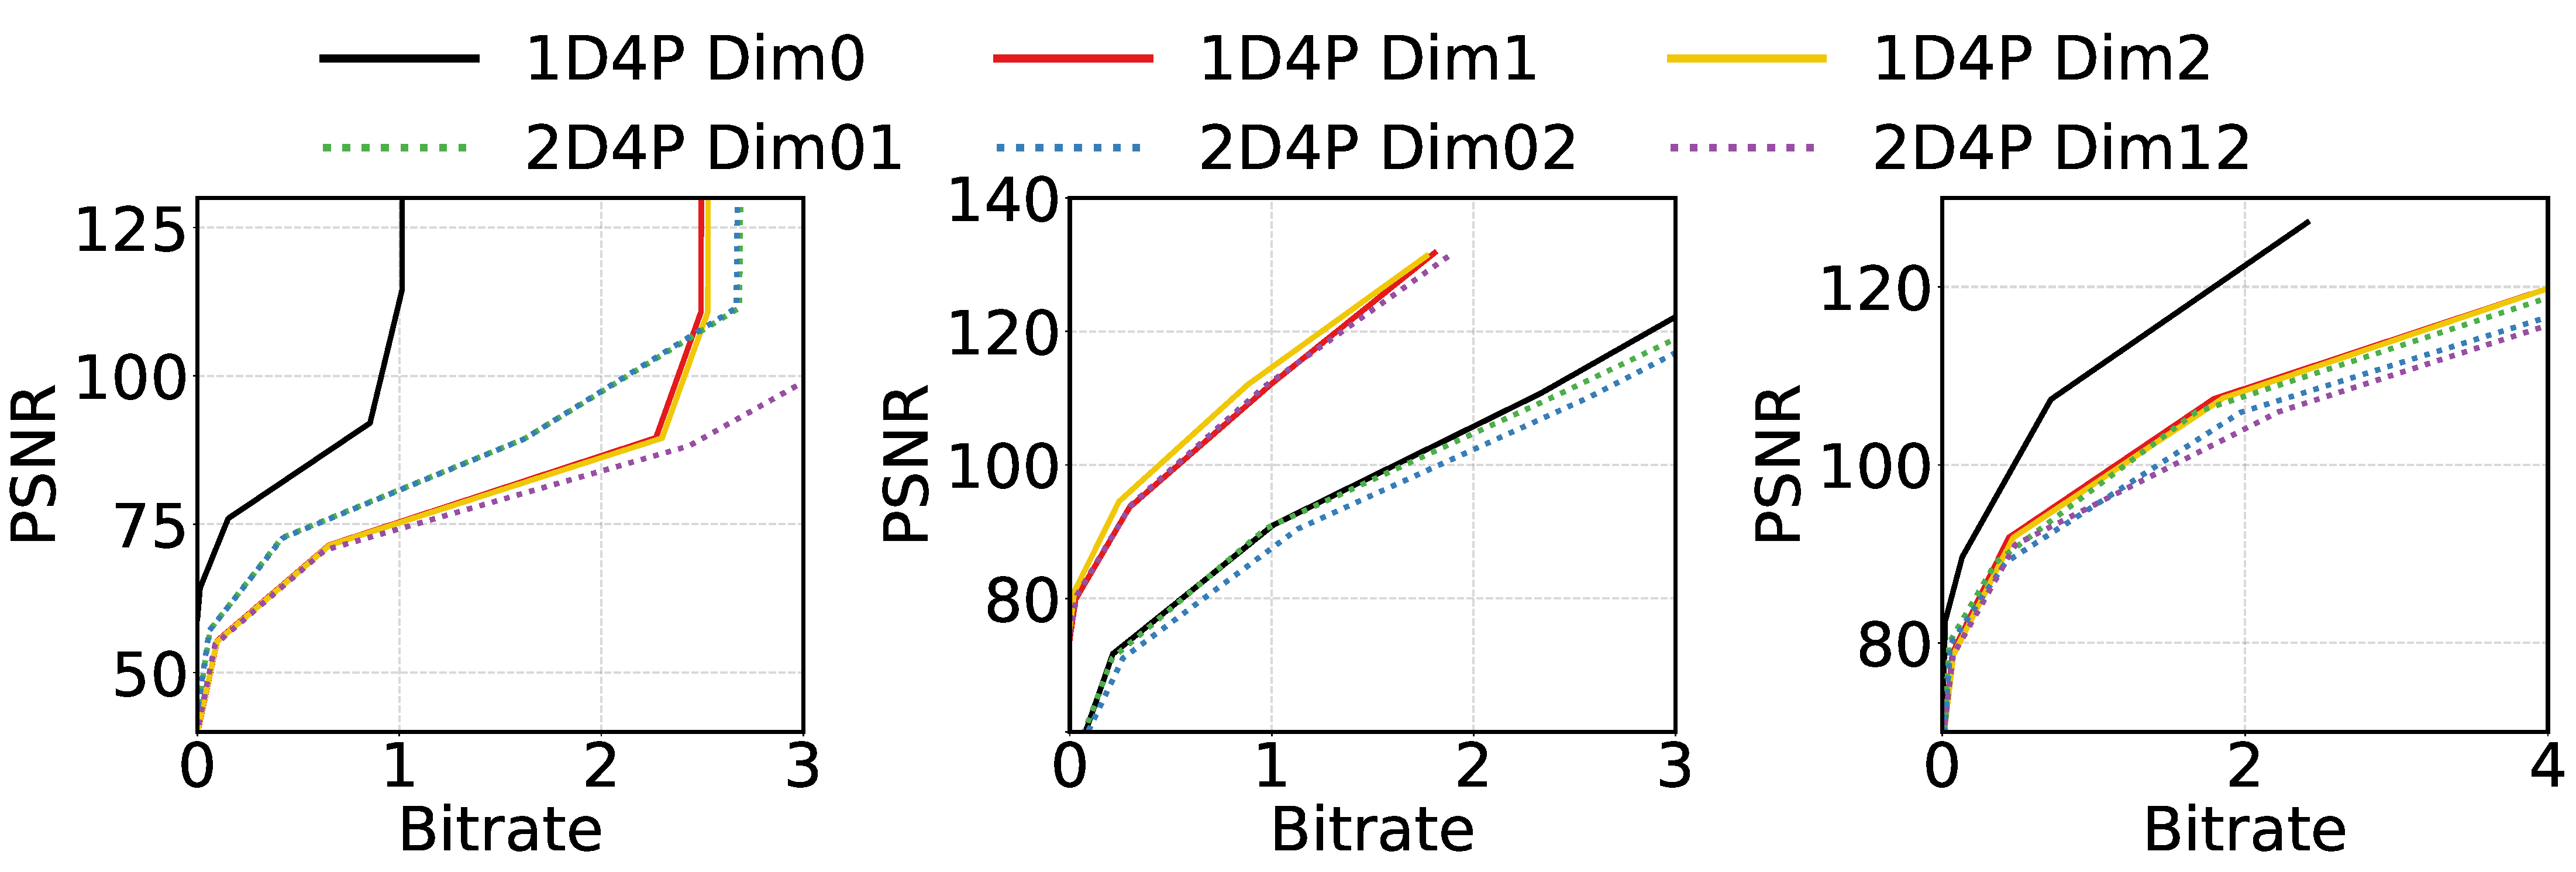
\includegraphics[width=1\linewidth]{figs/3/1D4和2D4对比.pdf}
    \caption{Rate distortion curve (with PSNR) for 1D and 2D interpolation predictor. xDyP here indicates x-dimensionality with y data points used for prediction. The lower bitrate and the higher PSNR, the better performance for a compressor.}
    \label{fig:1d-is-better-than-2d}
\end{figure}

% 我们在多个数据集上的测试结果验证了我们先前的推理。最好的1D四点预测器总是好过最好的2D四点预测器。类似的，从理论上我们也可以说明，在相同reference point数量的前提下，可变参数的1D预测器通常好过更高维的预测器。
Figure~\ref{fig:1d-is-better-than-2d} compares the rate–distortion performance of 1D and 2D predictors across multiple datasets, including light source~\cite{huang2025lscomp} (left), weather simulation~\cite{kossin2004mesovortices} (middle), and climate simulation~\cite{kay2015community} (right).
Dimx denotes the specific dimension that is used for a 1D predictor, whereas Dimxy denotes the two dimensions that are used for a 2D predictor, resulting in 3 combinations in total.
For each dataset, the 1D predictors consistently achieve higher PSNR than the 2D predictors at the same bitrate.
Moreover, among different prediction directions, the best 1D predictor always outperforms the best 2D predictor.
These results indicate that, under the same number of reference points, increasing dimensionality does not necessarily improve prediction effectiveness.
Instead, the tunable 1D predictor is often sufficient to capture dominant data correlations and achieve better compression performance.


\begin{boxH}
\textbf{Observation 1:}
A tunable 1D predictor is sufficient and often more effective than tunable 2D predictors.
\end{boxH}



\subsection{Reference Points on Interpolation Coefficients}
% 用一些实验证明，4个reference point就够了。再多，有benefit，但是coefficients search的代价太大了，得不偿失。
% 简而言之，得到takeaway2：4个reference points就够用了！

% 运行速度线性增长，搜索空间指数级增长，导致搜索时间也指数级增长，但效果没有增加太多（需要实验证明）

% 在前一个subsection中，我们验证了计算量大致相等的情况。这里我们比较一下1D4点可变参数预测器（Figure 3（a））和与它在结构上相似的两种1D6点可变参数预测器。
In Section~\ref{sec:stencil-patterns-performance}, we compared predictors with different dimensionality.
Here, we investigate how the number of reference points affects prediction performance.
Figure~\ref{fig:six-datapoints-1d-prediction} shows the coefficients of the 1D predictors with six reference points.
Each six-point predictor extends the four-point predictor by including additional reference points.
As a result, its parameter space strictly generalizes that of the four-point predictor.
This allows the six-point predictor to achieve compression no worse than the four-point predictor, theoretically.

\begin{figure}[htb]
    \centering
    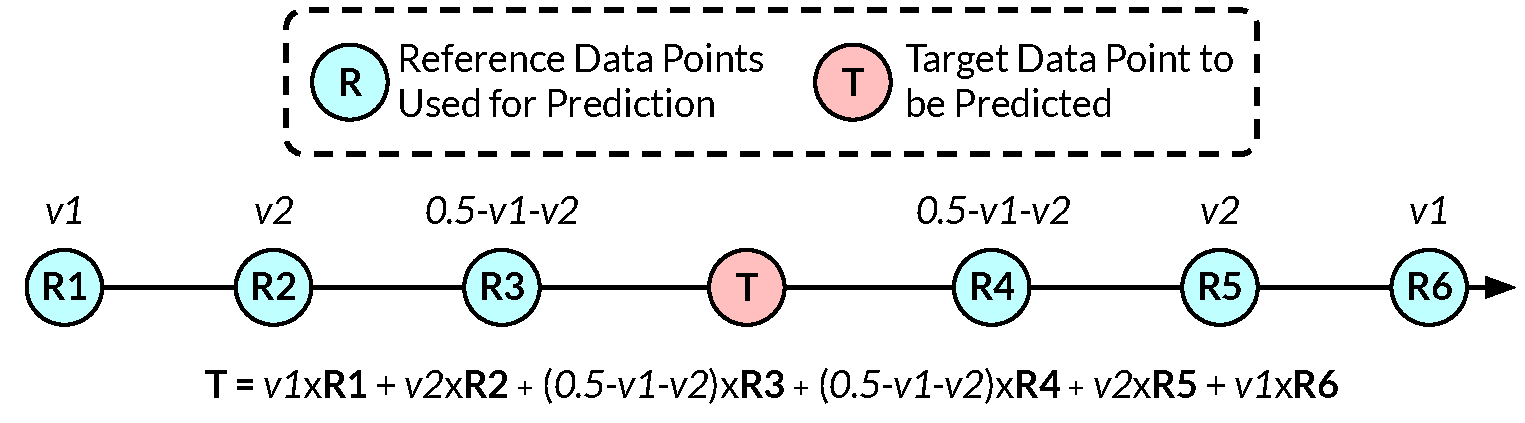
\includegraphics[width=1\linewidth]{revised-fig/3-six-coefficients-and-tunable-variables.pdf}
    \caption{1D interpolation predictor with 6 reference data points.}
    \label{fig:six-datapoints-1d-prediction}
\end{figure}

% 在Figure X中，我们展示了两种6点预测器的参数设计，它们的reference point都包含了1D4点预测器的reference point。由于参数是可变的，它们的搜索空间包含了1D四点预测器的搜索空间，所以压缩效果一定不会弱于1D4点预测器


% 如果在这两种预测器上使用五阶插值来求出coefficients，那么coefficients从近到远分别是Figure X（a）的15/20,-6/20,1/20和Figure X（b）的150/256,-25/256,3/256。我们让coefficients在一阶插值到五阶插值之间变动。
Figure~\ref{fig:six-datapoints-1d-prediction} shows our 1D six-point predictor pattern, which is inherited from the design in QoZ.
Six reference data points around the target points are used, and symmetric coefficients are assigned to the two sides.
We introduce two tunable variables, $v_1$ and $v_2$, to control the coefficients of the outer reference points.
The remaining coefficients are set to $0.5-v_1-v_2$, which ensures that all coefficients sum to 1.
Specifically, the predicted value is computed as
\[
T =
v_1(R_1+R_6) + v_2(R_2+R_5) + (0.5-v_1-v_2)(R_3+R_4).
\]
This formulation allows the predictor to adjust the relative contribution of near and far reference points while preserving coefficient normalization.
If the coefficients are instantiated from quintic interpolation, the three coefficients from near to far are
$\frac{15}{20}$, $-\frac{6}{20}$, and $\frac{1}{20}$.
This setting of coefficients corresponds to fixed interpolation predictors, while our formulation treats the coefficients as tunable parameters.

\begin{figure}[htb]
    \centering
    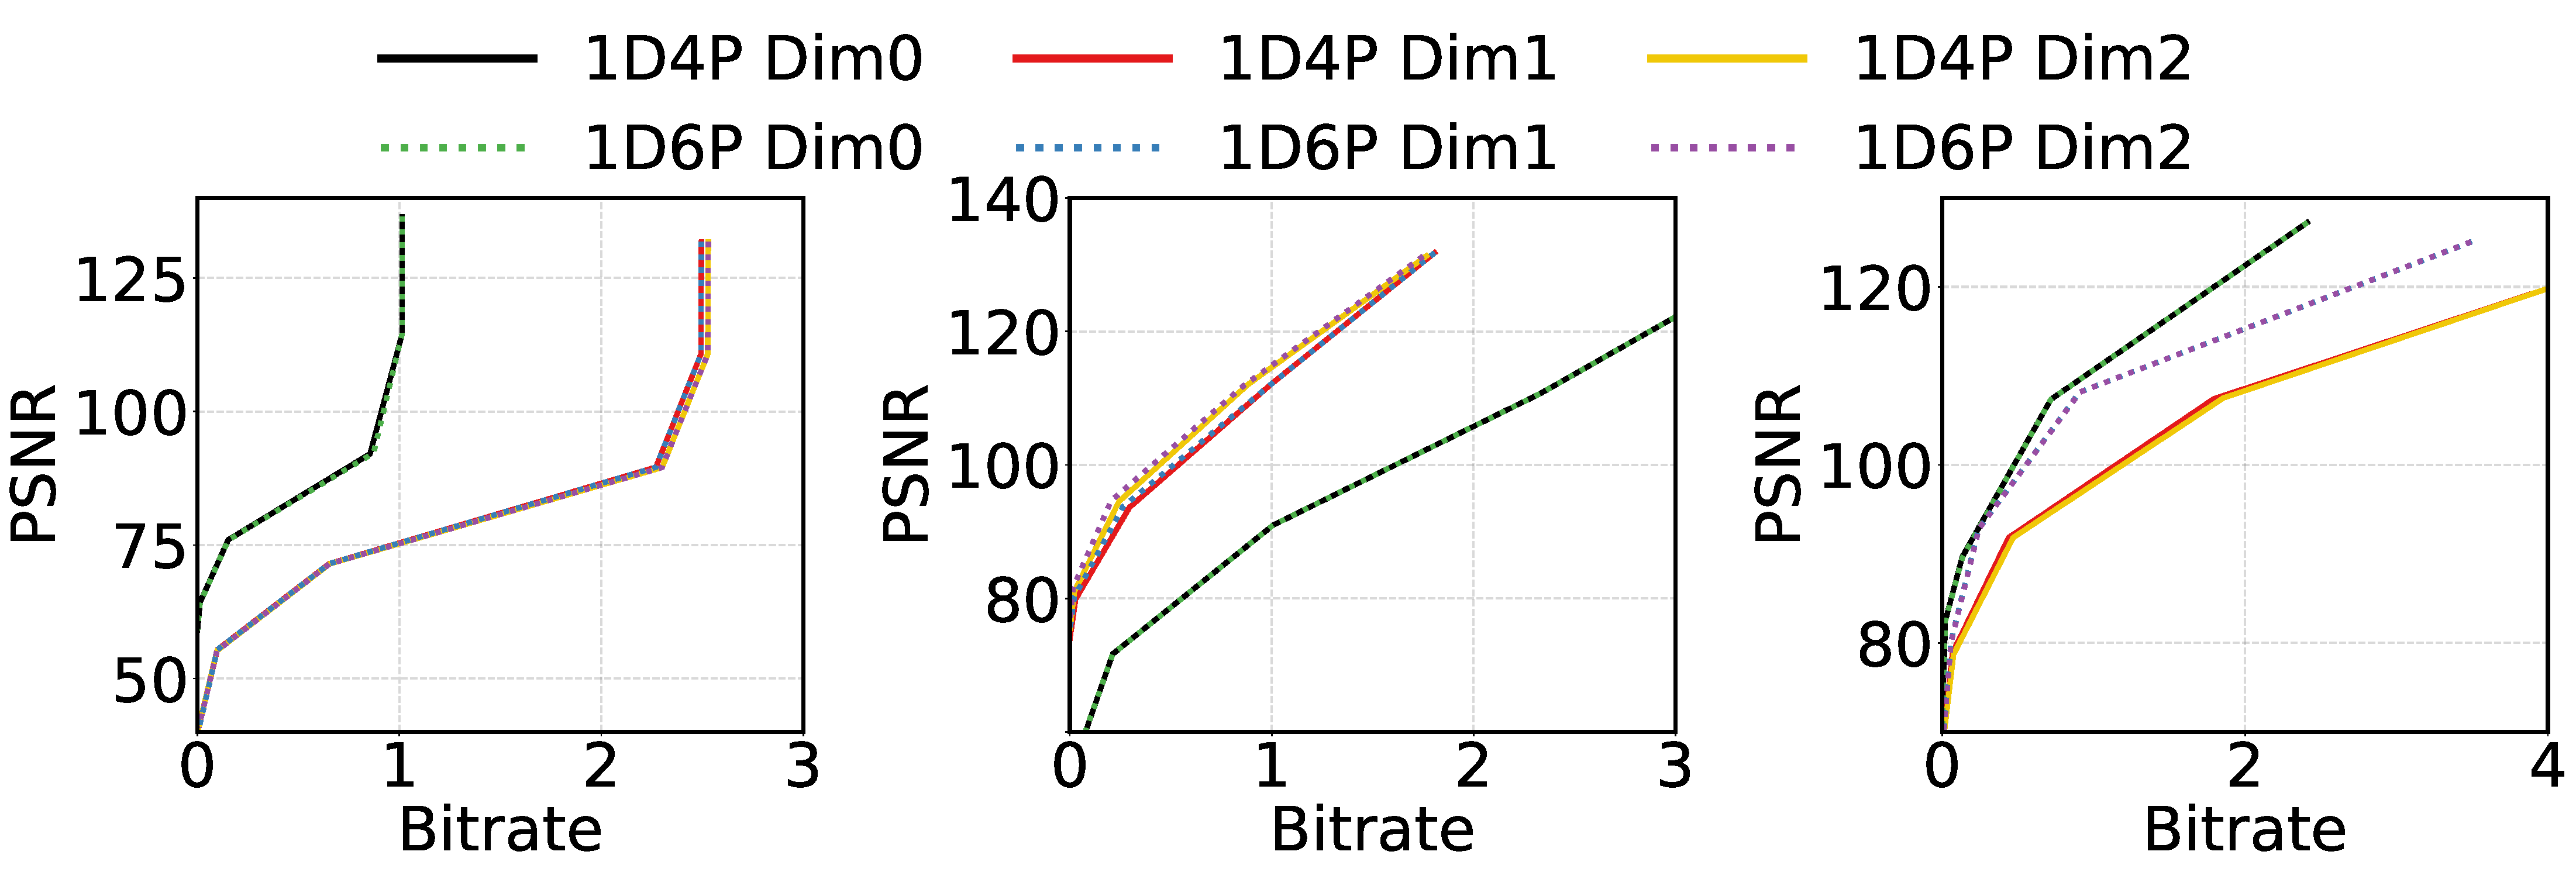
\includegraphics[width=1\linewidth]{figs/3/1D4和1D6对比.pdf}
    \caption{Rate distortion curve (with PSNR) for 1D interpolation predictor with different number of reference data points (4 or 6). Dim0, Dim1, or Dim3 denote the dimension that is used to perform prediction in an original 3D HPC field.}
    \label{fig:four-vs-six-results}
\end{figure}

Figure~\ref{fig:four-vs-six-results} compares the PSNR-based rate–distortion performance of 1D predictors with four and six reference points.
The HPC datasets~\cite{huang2025lscomp,kossin2004mesovortices,kay2015community} we used are consistent with Figure~\ref{fig:1d-is-better-than-2d}.
Across all datasets and prediction directions, the six-point predictors achieve only marginal improvement over the four-point predictors, and in many cases the two curves largely overlap.
This limited gain suggests that incorporating additional reference points does not improve prediction quality.
Meanwhile, increasing the number of reference points introduces higher implementation overhead and substantially enlarges the search space for coefficient tuning.
% Based on this trade-off, we adopt the four-point predictor in the remainder of this work.

\begin{boxH}
\textbf{Observation 2:}
Using four reference points is sufficient to achieve strong compression performance.
\end{boxH}